\section{Ejercicio 1}

\subsection{Consigna}

\textbf{Consigna:} Entrene una red de Hopfield '82 con las imágenes binarias disponibles en el campus.

\begin{enumerate}
	\item[\textbf{a)}] Verifique si la red aprendió las imágenes enseñadas.
	
	\item[\textbf{b)}] Evalúe la evolución de la red al presentarle versiones alteradas de las imágenes aprendidas: agregado de ruido, elementos borrados o agregados.
	
	\item[\textbf{c)}] Evalúe la existencia de estados espurios en la red: patrones inversos y combinaciones de un número impar de patrones. (Ver \textit{Spurious States}, en la sección 2.2, Hertz, Krogh \& Palmer, pág. 24).
	
	\item[\textbf{d)}] Realice un entrenamiento con las 6 imágenes disponibles. ¿Es capaz la red de aprender todas las imágenes? Explique.
\end{enumerate}

\subsection{Resolución}

\subsubsection{Preprocesamiento}

Una limitación estructural fundamental de la red de Hopfield es la imposibilidad de memorizar o procesar patrones (imágenes) de diferentes tamaños de forma simultánea. Esta restricción se debe directamente a la formulación matemática de su arquitectura:

La red está definida por una cantidad estática y fija de $N$ neuronas. Cada imagen bidimensional que se presenta a la red debe ``aplanarse'' previamente hasta convertirse en un vector unidimensional de estado $\xi^\mu$ de longitud $N$. Consecuentemente, la matriz de pesos sinápticos $w_{ij}$, encargada de almacenar los patrones mediante las interconexiones, posee un tamaño estricto y predefinido de $N \times N$.

Teniendo en cuenta que el set de imágenes provisto por la catedra contenía ejemplares de distintos tamaños, el primer paso fue seleccionar un \textit{subset} de imagenes del mismo tamaño. En este caso se seleccionaron las tres imagenes de tamaño $50 \times 50$ píxeles. Una vez aplanadas las imágenes en patrones de 2500 posiciones, ya estaban listas para entrenar a la red.

\subsubsection{Verificación de entrenamiento}
El siguiente paso fue verificar que la red había aprendido los patrones con los que fue entrenados correctamente. El resultado se puede observar en la figura \ref{fig:1_a}. Efectivamente, aprendió los patrones ya que no modificó las imagenes que se le pasaron.

\begin{figure}[htbp]
	\centering
	
	% --- Primera sub-imagen ---
	\begin{subfigure}[b]{0.32\textwidth}
		\centering
		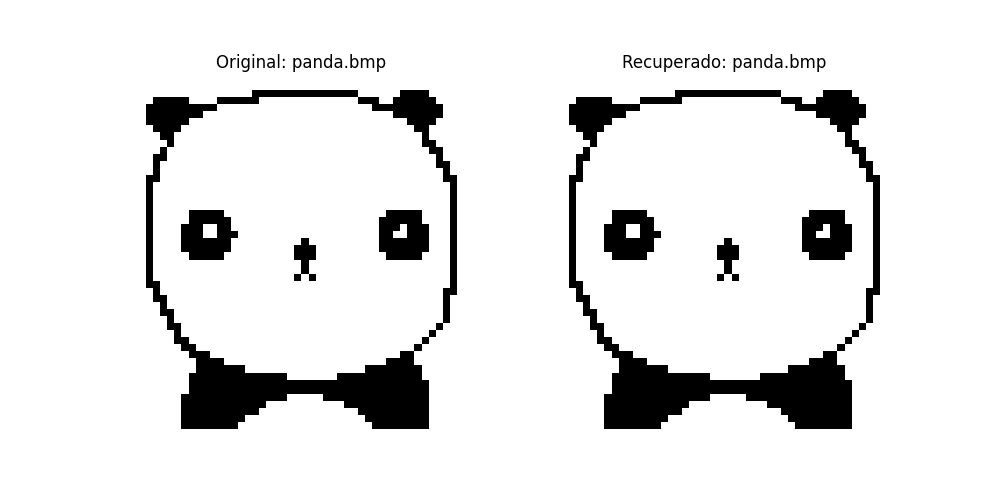
\includegraphics[width=\textwidth]{img_informe/panda_original_recuperado.png}
		\caption{Panda original vs. red.}
		\label{fig:panda_original_recuperado}
	\end{subfigure}
	\hfill % Espacio horizontal flexible para separar las imágenes
	% --- Segunda sub-imagen ---
	\begin{subfigure}[b]{0.32\textwidth}
		\centering
		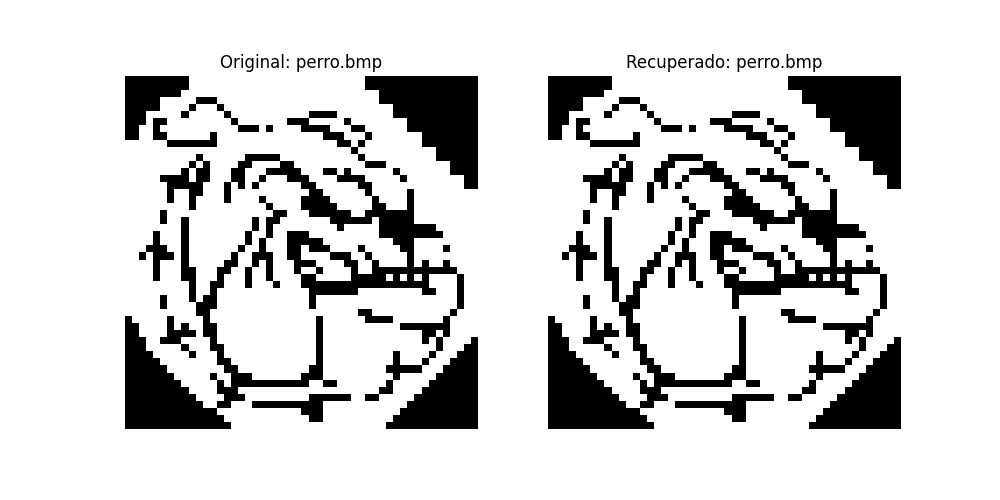
\includegraphics[width=\textwidth]{img_informe/perro_original_recuperado.png}
		\caption{Perro original vs. red.}
		\label{fig:perro_original_recuperado}
	\end{subfigure}
	\hfill % Espacio horizontal flexible
	% --- Tercera sub-imagen ---
	\begin{subfigure}[b]{0.32\textwidth}
		\centering
		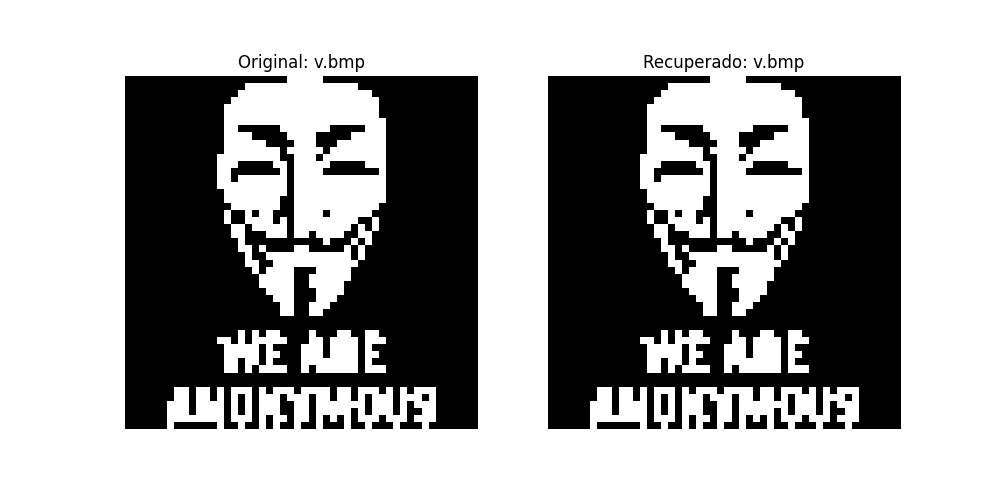
\includegraphics[width=\textwidth]{img_informe/v_original_recuperado.png}
		\caption{Imágen 'v' original vs. red.}
		\label{fig:v_original_recuperado}
	\end{subfigure}
	
	% --- Caption y Label de la figura general ---
	\caption{Comparación entre las imágenes originales y las que devuelve la red.}
	\label{fig:1_a}
\end{figure}


\subsubsection{Patrones alterados}
La próxima prueba para la red fue intentar recuperar las imágenes con las que fue entrenada, a partir de esos mismos patrones, pero alterados. La manera de probar esto fue implementar una modificación distinta a cada imágen y ver que tanto se la podía modificar antes de que la red falle en recuperar el patrón original.

En primer lugar se probó borrando las esquinas de la imagen \textbf{v.bmp}. Los resultados se pueden observar en la figura \ref{fig:1_b_v}. Se puede ver como en el primer caso la red puede recuperar la imagen, sin embargo en el segundo caso no. A priori este resultado tiene sentido, ya que durante el entrenamiento quedó plasmada la relación entre los píxeles del fondo de la imagen. Cuando la red ve que las esquinas están un poco blancas, pero todo lo demás está negro, oscurece el blanco acorde a los pesos entre neuronas aprendidos en el entrenamiento. En el segundo caso, al haber tanto blanco, la red vira hacia la imagen con más blanco con la que fue entrenada, el panda. También es importante notar como siempre cambia todo lo necesario en la primer iteración, mientras que la segunda solamente sirve para confirmar que no hay ningún otro cambio para hacer.



\begin{figure}[htbp]
	\centering
	
	% --- Primera sub-imagen (esquinas 10) ---
	\begin{subfigure}[b]{0.48\textwidth}
		\centering
		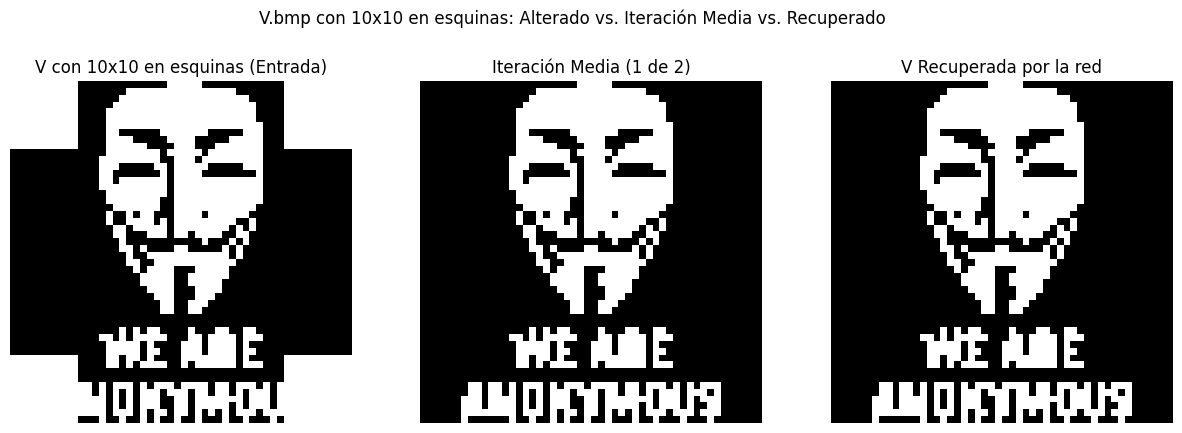
\includegraphics[width=\textwidth]{img_informe/v_esquinas_10_entrada_parcial_salida.png}
		\caption{Borradas con 10 píxeles de lado.}
		\label{fig:v_esquinas_10}
	\end{subfigure}
	\hfill % Espacio horizontal flexible para separar las imágenes
	% --- Segunda sub-imagen (esquinas 20) ---
	\begin{subfigure}[b]{0.48\textwidth}
		\centering
		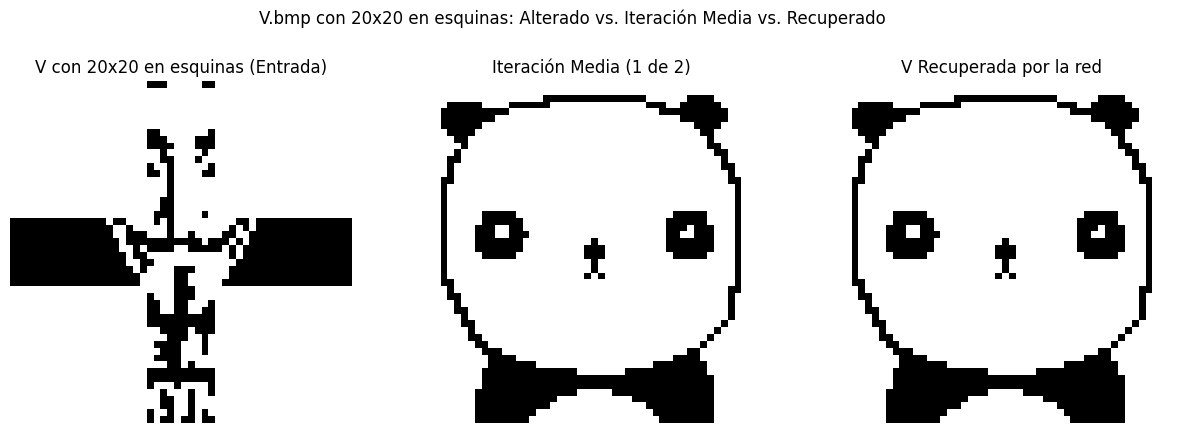
\includegraphics[width=\textwidth]{img_informe/v_esquinas_20_entrada_parcial_salida.png}
		\caption{Borradas con 20 píxeles de lado.}
		\label{fig:v_esquinas_20}
	\end{subfigure}
	
	% --- Caption y Label de la figura general ---
	\caption{Performance de la red ante borrado de las esquinas en diferentes medidas.}
	\label{fig:1_b_v}
\end{figure}

Otra prueba que se realizó fue pintar las diagonales de la imagen del perro, al igual que en el caso anterior, con diferentes grosores. Los resultados se pueden observar en la figura \ref{fig:1_b_perro}. Similarmente, el primer grosor lo soporta correctamente, devolviendo la imagen original. El segundo caso es más complicado, ya que no recupera la original pero tampoco recupera otro patrón con el que haya sido entrenado. El prestar mucha atención, se puede observar que termina en una combinación de las tres imágenes y con colores invertidos. Esto es un estado espurio, tema que se desarrollará más adelante.

\begin{figure}[htbp]
	\centering
	
	% --- Primera sub-imagen (diagonal 8) ---
	\begin{subfigure}[b]{0.48\textwidth}
		\centering
		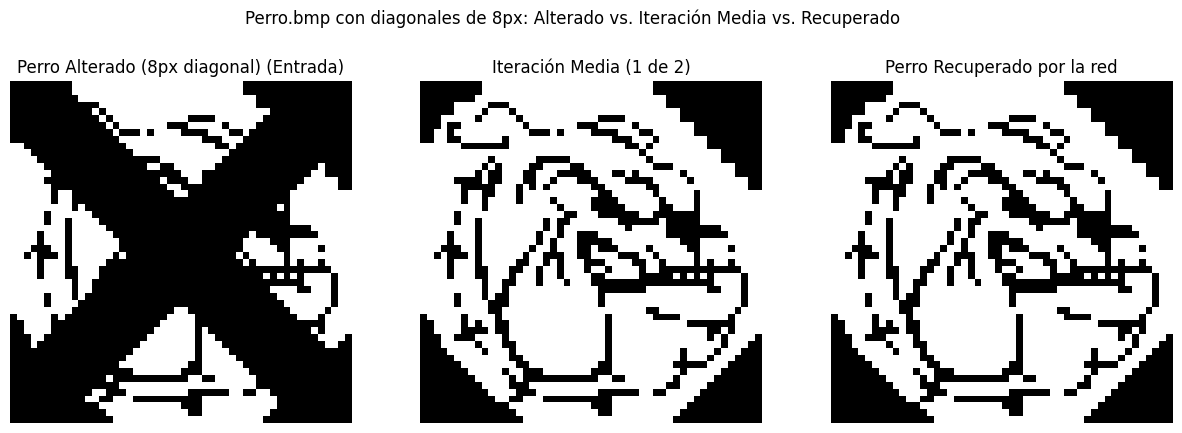
\includegraphics[width=\textwidth]{img_informe/perro_diagonal_8_entrada_parcial_salida.png}
		\caption{Diagonales con 8 píxeles de grosor.}
		\label{fig:perro_diagonal_8}
	\end{subfigure}
	\hfill % Espacio horizontal flexible para separar las imágenes
	% --- Segunda sub-imagen (diagonal 10) ---
	\begin{subfigure}[b]{0.48\textwidth}
		\centering
		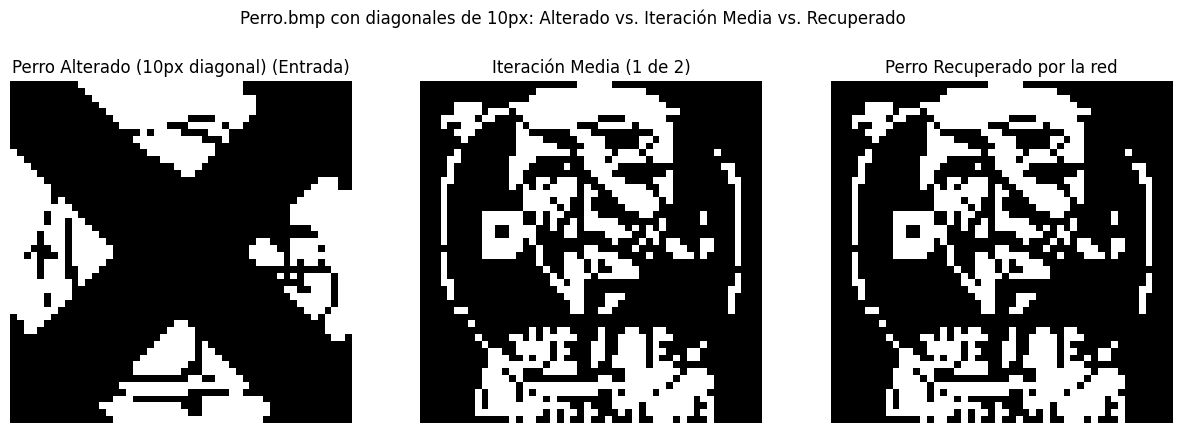
\includegraphics[width=\textwidth]{img_informe/perro_diagonal_10_entrada_parcial_salida.png}
		\caption{Diagonales con 10 píxeles de grosor.}
		\label{fig:perro_diagonal_10}
	\end{subfigure}
	
	% --- Caption y Label de la figura general ---
	\caption{Performance de la red ante pintado de las diagonales con distintos grosores.}
	\label{fig:1_b_perro}
\end{figure}

Para la tercer y última imagen con la que la red fue entrenada, se introdujo distintas cantidades de ruido para ver como recuperaba las imagenes. Estos resultados se pueden ver en la figura \ref{fig:1_b_panda}. La transición se da exactamente igual que en los casos anteriores, solamente con un intermedio. De la misma manera que en las anteriores, existe un umbral donde el ruido es tanto que interpreta afinidad con otro patrón. La imagen del panda es mayoritariamente blanca, pero con $50\%$ de ruido se torna bastante oscura, razón por la que la red la confunde con la imagen \textbf{v.bmp}.

\begin{figure}[htbp]
	\centering
	
	% --- Primera sub-imagen (ruido 30%) ---
	\begin{subfigure}[b]{0.48\textwidth}
		\centering
		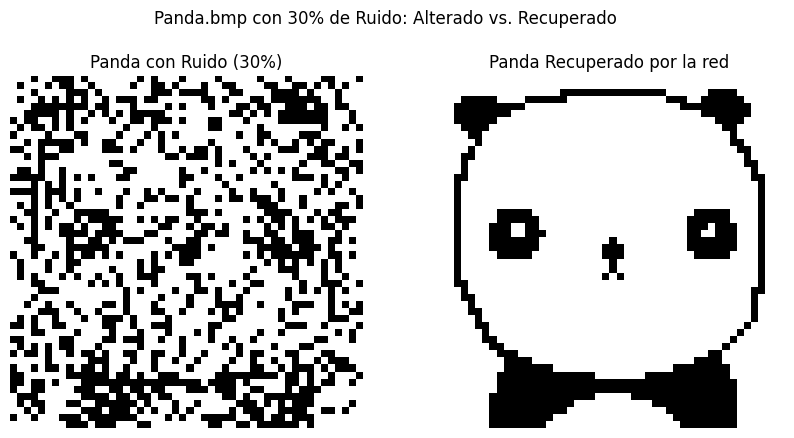
\includegraphics[width=\textwidth]{img_informe/ruido_30_panda.png}
		\caption{Ruido del 30\% en los píxeles.}
		\label{fig:ruido_30_panda}
	\end{subfigure}
	\hfill % Espacio horizontal flexible para separar las imágenes
	% --- Segunda sub-imagen (ruido 50%) ---
	\begin{subfigure}[b]{0.48\textwidth}
		\centering
		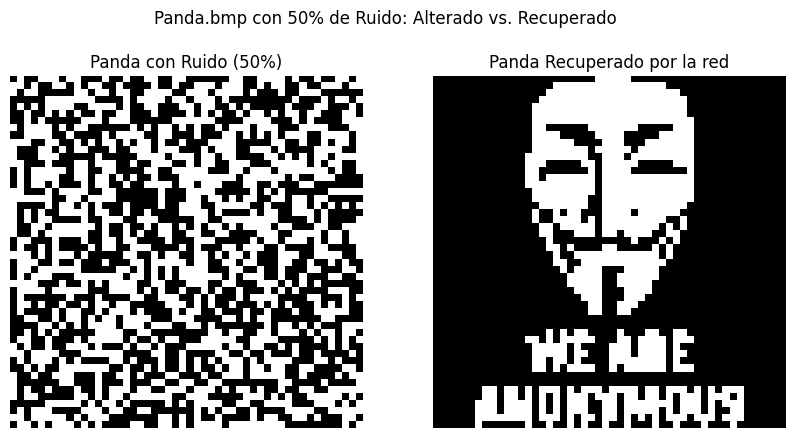
\includegraphics[width=\textwidth]{img_informe/ruido_50_panda.png}
		\caption{Ruido del 50\% en los píxeles.}
		\label{fig:ruido_50_panda}
	\end{subfigure}
	
	% --- Caption y Label de la figura general ---
	\caption{Performance de la red ante ruido en los píxeles.}
	\label{fig:1_b_panda}
\end{figure}

\subsubsection{Estados espurios}

En el ejemplo del perro con las diagonales pintadas se tuvo un primer acercamiento al fenómeno de los estados espurios. Como se menciona en la sección \ref{sec:intro} los estados espurios pueden ser los mismos patrones invertidos o una mezcla impar de patrones. Para demostrar la existencia de los estados mencionados, se le entregó a la red la imagen del panda con los colores invertidos. El resultado fue el esperado, la red convergió a la misma imagen que le fue entregada (figura \ref{fig:panda_invertido}). Cabe aclarar que solamente le tomó una iteración, es decir, no efectuó cambios. También pueden pasar cosas más complejas, como se obervó en la figura \ref{fig:perro_diagonal_10}, donde el resultado es una suerte de combinación de los tres patrones y al mismo tiempo con colores invertidos.

Los estados espurios también pueden generarse como una suma impar de estados aprendidos por la red. Para probar esto, se generó un estado espurio a partir de las tres imagenes y se lo entregó a la red para observar la salida. Teóricamente, este estado debería ser estable, por lo que la salida sería igual a la entrada. En la figura \ref{fig:estado_espurio} se observa como efectivamente la red no modifica ningún píxel.

\begin{figure}[htbp]
	\centering
	
	% --- Primera sub-imagen (Panda invertido) ---
	\begin{subfigure}[b]{0.48\textwidth}
		\centering
		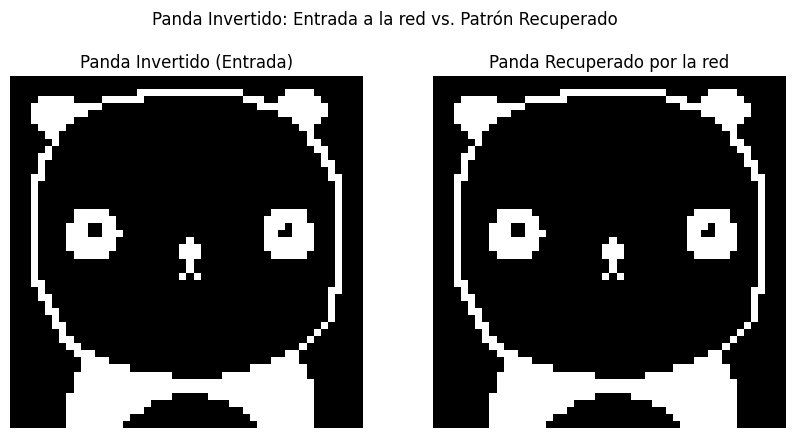
\includegraphics[width=\textwidth]{img_informe/panda_invertido}
		\caption{Rendimiento ante un patrón invertido.}
		\label{fig:panda_invertido}
	\end{subfigure}
	\hfill % Espacio horizontal flexible para separar las imágenes
	% --- Segunda sub-imagen (Estado espurio) ---
	\begin{subfigure}[b]{0.48\textwidth}
		\centering
		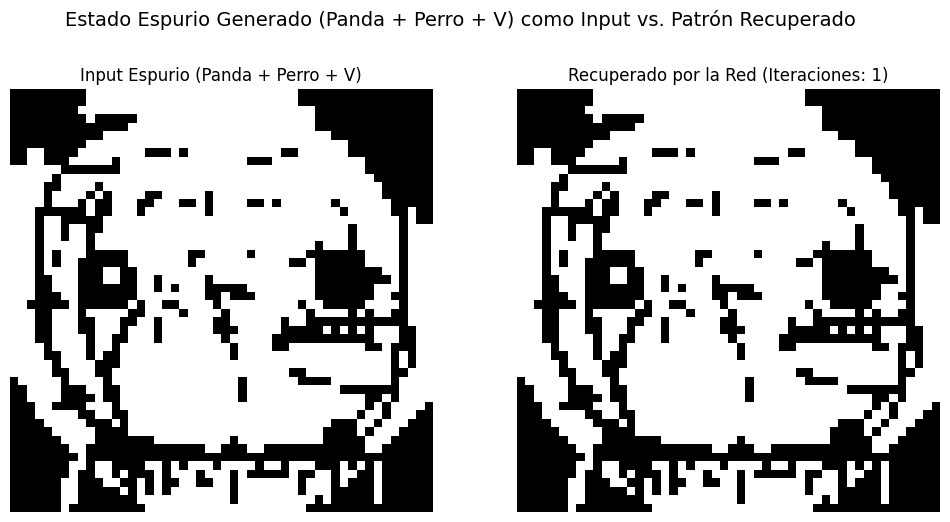
\includegraphics[width=\textwidth]{img_informe/estado_espurio.png}
		\caption{Rendimiento ante un estado espurio.}
		\label{fig:estado_espurio}
	\end{subfigure}
	
	% --- Caption y Label de la figura general ---
	\caption{Análisis de los estados espurios en la red.}
	\label{fig:analisis_estados_espurios}
\end{figure}

\subsubsection{Entrenamiento de la red con los 6 patrones}

Por último, adaptaron los tamaños de las 3 imagenes restantes del \textit{dataset}, para lograr una misma cantidad de neuronas que las imagenes ya usadas. La figura \ref{fig:train_6} muestra como hubo algunos patrones que la red no pudo aprender correctamente. Esto puede ser por similaridad de colores con otra imagen, por ejemplo la paloma y el panda.

\begin{figure}[htbp]
	\centering
	
	% --- Primera sub-imagen ---
	\begin{subfigure}[b]{0.8\textwidth}
		\centering
		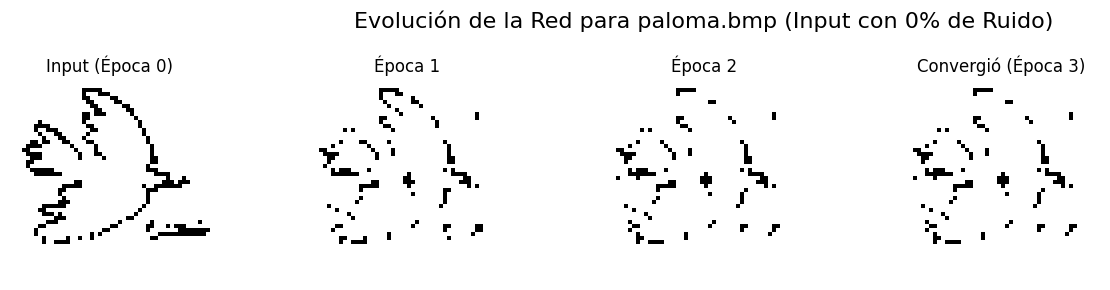
\includegraphics[width=\textwidth]{img_informe/paloma_6.png}
		\caption{Evolución de la red frente a la paloma.}
		\label{fig:paloma_6}
	\end{subfigure}
	
	\vspace{0.5cm} % Espacio vertical para que no queden pegadas
	
	% --- Segunda sub-imagen ---
	\begin{subfigure}[b]{0.8\textwidth}
		\centering
		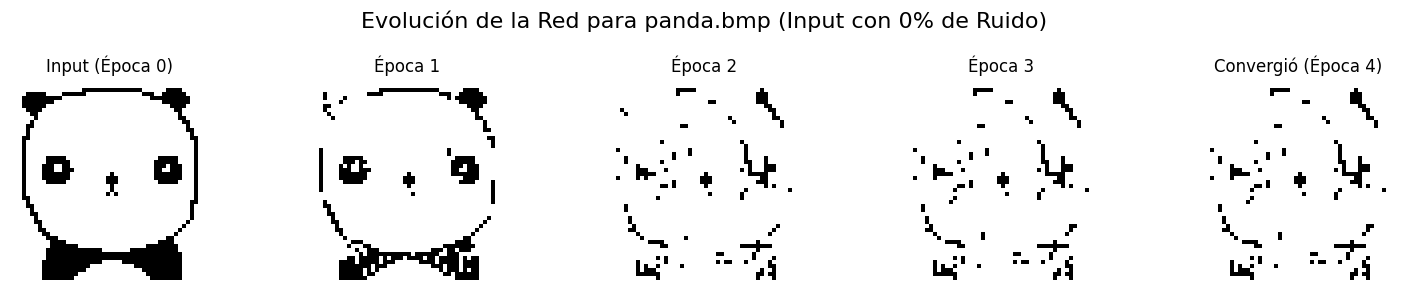
\includegraphics[width=\textwidth]{img_informe/panda_6.png}
		\caption{Evolución de la red ante el panda.}
		\label{fig:panda_6}
	\end{subfigure}

	
	
	% --- Caption y Label de la figura general ---
	\caption{Rendimiento de la red con entrenamiento de 6 imágenes.}
	\label{fig:train_6}
\end{figure}

